\documentclass[11pt]{article}
\usepackage{fontspec}
\ifdefined\PortableFonts
  \setmainfont{texgyretermes-regular.otf}[BoldFont=texgyretermes-bold.otf,ItalicFont=texgyretermes-italic.otf,BoldItalicFont=texgyretermes-bolditalic.otf]
\else
  \setmainfont{Times New Roman}
\fi
\setmonofont{lmmono10-regular.otf}[Scale=MatchLowercase]
\usepackage{amsmath,amsthm}
\usepackage{unicode-math}
\setmathfont{texgyretermes-math.otf}
\usepackage[paperwidth=5.5in,paperheight=8.5in,textwidth=4.9in,textheight=7.7in,centering,noheadfoot]{geometry}
\usepackage{graphicx,booktabs,caption,needspace,placeins}
\usepackage{titlesec}
\titleformat{\section}{\normalfont\bfseries\fontsize{12}{14}\selectfont}{\thesection.}{0.5em}{}
\titleformat{\subsection}{\normalfont\bfseries}{\thesubsection.}{0.5em}{}
\titlespacing*{\section}{0pt}{13pt plus 2pt minus 2pt}{6pt}
\titlespacing*{\subsection}{0pt}{10pt plus 2pt minus 1pt}{4pt}
\usepackage[hidelinks,unicode]{hyperref}
\usepackage{url}
\urlstyle{same}
\captionsetup{font=normalsize,labelfont=bf,labelsep=period,skip=6pt,justification=justified,singlelinecheck=false}
\pagestyle{empty}
\makeatletter
\renewcommand\normalsize{\@setfontsize\normalsize{11pt}{13.2pt}%
  \abovedisplayskip 9pt plus 2pt minus 3pt
  \abovedisplayshortskip 0pt plus 3pt
  \belowdisplayshortskip 6pt plus 3pt minus 3pt
  \belowdisplayskip \abovedisplayskip}
\makeatother
\normalsize
\setlength{\parindent}{1em}
\setlength{\parskip}{0pt plus 0.4pt}
\setlength{\textfloatsep}{12pt plus 2pt minus 2pt}
\setlength{\intextsep}{12pt plus 2pt minus 2pt}
\setlength{\floatsep}{10pt}
\renewcommand{\topfraction}{0.9}
\renewcommand{\bottomfraction}{0.8}
\renewcommand{\textfraction}{0.08}
\renewcommand{\floatpagefraction}{0.7}
\setcounter{topnumber}{2}
\emergencystretch=1.8em
\widowpenalty=10000
\clubpenalty=10000
\displaywidowpenalty=10000
\brokenpenalty=10000
\raggedbottom
\newcommand{\R}{\mathbb R}
\newcommand{\Q}{\mathbb Q}
\newcommand{\disk}{D}
\newcommand{\area}{\operatorname{area}}
\newcommand{\suppfile}[1]{\path{#1}}
\newtheoremstyle{paperthm}{6pt}{6pt}{\normalfont}{}{\bfseries}{.}{0.5em}{}
\theoremstyle{paperthm}

\usepackage{xeCJK}
\setCJKmainfont{SimSun}[BoldFont=SimHei,ItalicFont=KaiTi]
\setCJKsansfont{SimHei}
\setCJKmonofont{SimSun}
\renewcommand{\figurename}{图}
\renewcommand{\refname}{参考文献}
\renewcommand{\proofname}{证明}
\newtheorem{theorem}{定理}
\newtheorem{lemma}{引理}
\newtheorem{proposition}{命题}
\hypersetup{pdftitle={圆内68个单位正方形装箱的严格上下界},pdfauthor={张世逸},pdfsubject={精确构造与计算机辅助下界证明}}
\begin{document}
\begin{center}
{\fontsize{14}{17}\selectfont\bfseries 圆内68个单位正方形装箱的严格上下界\par}
\vspace{7pt}
{\fontsize{12}{14}\selectfont 张世逸\par}
\vspace{3pt}
上海大学；\href{mailto:chromoany@Gmail.com}{chromoany@Gmail.com}
\end{center}
\vspace{5pt}
\noindent\textbf{摘要.}
设 $r(68)$ 为容纳68个单位正方形的可行圆盘半径的下确界，正方形可任意旋转，内部两两不交。本文给出一个有理坐标构造，并利用计算机辅助排除证明
\[
\frac{39}{8}<r(68)<5.031404629453352.
\]
构造的包围半径由一个整数系数二次方程及宽度为 $10^{-30}$ 的隔离区间精确确定。下界采用定义在80个同心圆环上的非负径向权函数，通过对连续二维参数域的完整划分，以精确有理运算和外包区间验证单块积分不等式。随文提供完整坐标、权重、划分数据和验证程序。全局精确最优值以及半径为5时能否容纳68块，仍未确定。

\medskip
\noindent\textbf{关键词.} 正方形装箱；圆盘；精确构造；加权面积；计算机辅助证明。

\section{问题与主要结果}
记 $D_R=\{z\in\R^2:\|z\|\le R\}$。所考虑的装法由闭单位正方形组成，其内部两两不交，边界允许相切，各块均可自由平移和旋转。把外圆圆心平移至原点不限制一般性。定义 $r(68)$ 为所有可行半径的下确界。

\begin{theorem}\label{thm:main}
存在一个明确给出的68块装法，各块的中心与单位方向向量均为有理数。记该装法关于指定原点的包围半径为 $\widehat R$，则
\begin{equation}\label{eq:bounds}
\frac{39}{8}<r(68)\le\widehat R<U,
\qquad U=\frac{5031404629453352}{10^{15}}.
\end{equation}
并且
\begin{equation}\label{eq:isolation}
\begin{gathered}
5.031404629453350730787899409097
<\widehat R,\\
\widehat R<5.031404629453350730787899409098.
\end{gathered}
\end{equation}
\end{theorem}

Montanher等\cite{montanher}研究同一类允许自由旋转的圆内正方形装箱问题，并对三块情形的最优半径及构造给出严格区间包围。Domes与Neumaier\cite{domes}则讨论如何从近似解严格验证可行性。在 $n=68$ 的直接历史对照中，Jelliss\cite{jelliss}给出半径为 $\sqrt{26}$ 的网格构造。由于 $U^2<26$，式\eqref{eq:bounds}的上界严格小于这一历史值；此比较不构成当前世界纪录或文献优先权的声明。

初等面积下界为 $r(68)\ge\sqrt{68/\pi}\approx4.65242649$，本文将这一基线提高到严格下界 $39/8=4.875$。本文的贡献是一个明确的精确构造，以及覆盖所有实数姿态的可复现排除证书。Friedman的构造汇编\cite{friedman}提供了较小规模问题的背景；所查版本列至 $n=50$，并未提供 $n=68$ 的比较值。

下界方法为每个合法正方形分配一个最小加权面积。这类资源计数思路已有先例，例如Kearney与Shiu\cite{kearney}的不可避免集方法。Karakuş近期的预印本\cite{karakus}讨论了更一般的非负测度装箱界。本文的计数不等式本身是初等的；具体证书的作用在于，对圆盘内所有实数平移与转角验证同一个径向权函数。第\ref{sec:validation}节说明有限计算为何能够覆盖这一连续族。

\section{一个精确构造}
每块的数据由中心 $c_i\in\Q^2$ 和单位向量 $u_i\in\Q^2$ 给出，其中 $u_i\cdot u_i=1$。令 $v_i=(-u_{i,2},u_{i,1})$，四个顶点为
\begin{equation}\label{eq:vertices}
c_i+\frac{\varepsilon u_i+\eta v_i}{2},
\qquad \varepsilon,\eta\in\{-1,1\}.
\end{equation}
图\ref{fig:packing}展示该构造。内部主要呈列状排列，靠近圆周处有若干旋转方块组。装法由精确数据定义，绘图坐标仅用于显示。

\begin{figure}[htbp]
\centering
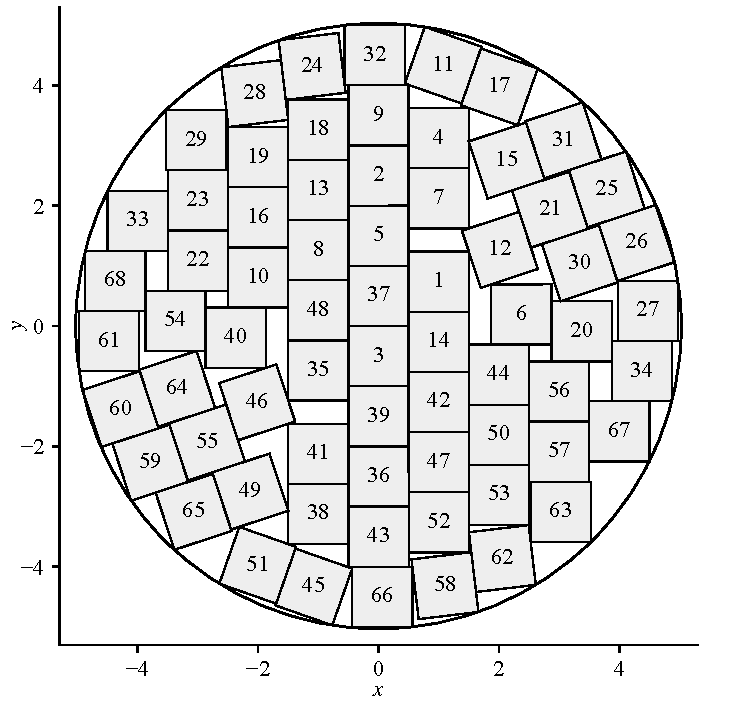
\includegraphics[width=\linewidth]{../../figures/packing-zh.pdf}
\caption{经认证的68块构造及其指定包围圆。编号与坐标文件中的方块编号一致。图中的浮点坐标仅用于显示。}\label{fig:packing}
\end{figure}

对任意一对 $i<j$，置
\[
H_{ij}=\frac{1+|u_i\cdot u_j|+|\det(u_i,u_j)|}{2}.
\]
在任一轴 $n\in\{u_i,v_i,u_j,v_j\}$ 上，$H_{ij}$ 都是两块投影半宽之和。因此，只要其中一条轴满足
\begin{equation}\label{eq:sat}
|(c_i-c_j)\cdot n|\ge H_{ij},
\end{equation}
两块的内部便不相交。反之，凸多边形的分离轴定理保证这四条轴已经足够；也可通过两块Minkowski差的边法向直接得到这一结论。式\eqref{eq:sat}允许等号，因而保留边界相切的情形。

随文验证器检查全部68个方向的单位长度、全部 $\binom{68}{2}=2278$ 对方块的式\eqref{eq:sat}，以及全部272个顶点的圆内包含关系。所有检查都是有理数比较，最终归结为整数运算。由 $D_U$ 的凸性，顶点包含推出整个方块包含。因此，上界不依赖几何容差，也不依赖产生该布局的数值搜索过程。

对互素正整数 $p,q$，此指定圆盘的精确半径为
\begin{equation}\label{eq:radius}
\widehat R=\sqrt{p/q},\qquad
\frac pq=\max_{i,\varepsilon,\eta}
\left\|c_i+\frac{\varepsilon u_i+\eta v_i}{2}\right\|^2,
\end{equation}
最大值仅在第25块的 $(\varepsilon,\eta)=(1,1)$ 顶点取得。$p,q$ 分别有1451位和1450位十进制数字，完整整数见补充材料\suppfile{upper/best-68-exact-radius.json}。方程 $qX^2-p=0$ 与式\eqref{eq:isolation}共同精确指定 $\widehat R$。将有理区间端点平方，即可严格验证式\eqref{eq:isolation}及 $\widehat R<U$。

这里的圆心是固定的，不主张它在允许移动圆心时仍是该点集的最小包围圆。因此，$qX^2-p$ 是图示构造的半径方程，并非未知全局最优值 $r(68)$ 的定义多项式。

\section{加权面积排除}\label{sec:weight}
置
\begin{equation}\label{eq:parameters}
s=\frac{40}{39},\qquad a=\frac{s}{2},\qquad
c=\frac{19926631}{20000000}.
\end{equation}
选取非负径向函数 $w$：当 $j/16\le\|z\|<(j+1)/16$ 时，其值为 $w_j\in\Q_{\ge0}$，其中 $j=0,\ldots,79$；在 $D_5$ 外取零。80个精确权重列于\suppfile{lower/weights.json}，图\ref{fig:weights}给出其形状。圆环边界上的取值不影响积分。

\begin{proposition}\label{prop:weight}
任意边长为 $s$ 且包含于 $D_5$ 的正方形 $S$，无论其实数中心与转角如何，均满足
\begin{equation}\label{eq:single}
\int_S w(\|z\|)\,dz\ge c.
\end{equation}
\end{proposition}

命题\ref{prop:weight}是计算机辅助验证的部分，其证书及各检查的数学依据见第\ref{sec:validation}节。

\begin{figure}[htbp]
\centering
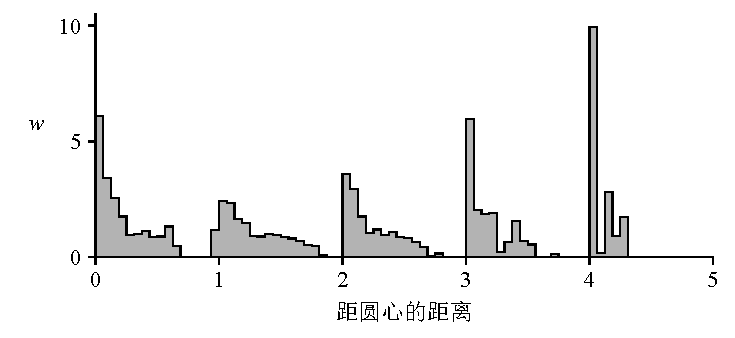
\includegraphics[width=\linewidth]{../../figures/weights-zh.pdf}
\caption{非负径向权函数。所有断点与高度均为有理数；积分计算完整保留了权重振荡产生的带符号差分。}\label{fig:weights}
\end{figure}

总权重为
\begin{equation}\label{eq:cost}
\begin{split}
C&=\int_{D_5}w(\|z\|)\,dz
 =\pi\sum_{j=0}^{79}w_j\frac{(j+1)^2-j^2}{256}\\
 &=\pi\frac{345050690237}{16000000000}
 <\frac{338752725}{5000000}
 <\frac{338752727}{5000000}=68c.
\end{split}
\end{equation}
其中第一个严格不等式只需
\[
\pi<P:=\frac{3141592653589794}{10^{15}}.
\]
由Machin恒等式
$\pi=16\arctan(1/5)-4\arctan(1/239)$ 及交错级数界即可得到它。具体地，令
\[
T(q,m)=\sum_{k=0}^{m}\frac{(-1)^k}{(2k+1)q^{2k+1}},
\]
则 $\pi<16T(5,12)-4T(239,3)<P$，后一个比较是精确有理运算。式\eqref{eq:cost}最后两个分数的差为 $1/2500000$。

若68个单位正方形能够装入半径不超过 $39/8$ 的圆盘，将整份装法按 $s=40/39$ 放大，便得到 $D_5$ 内68个边长为 $s$ 的正方形，且内部仍两两不交。它们的边界面积为零，非负性与命题\ref{prop:weight}于是给出
\[
68c\le\sum_{i=1}^{68}\int_{S_i}w
=\int_{\bigcup_i S_i}w\le C,
\]
与式\eqref{eq:cost}矛盾。

为了将排除结论转化为下确界的严格不等式，还须证明最小值取得。固定已知可行上端 $U$。每个单位正方形都包含以其中心为圆心、半径为 $1/2$ 的圆盘，因此 $D_U$ 中任一方块的中心范数不超过 $U-1/2$；方向向量位于紧致单位圆上。顶点包含条件为闭条件；内部不交由有限个闭条件\eqref{eq:sat}的析取表示，也为闭条件。所以，$D_U$ 内非空的可行参数集紧致，顶点范数的最大值作为连续函数在其上取得最小值。所有改善 $U$ 的装法都属于该集合，故此最小值正是 $r(68)$。已证明的排除于是给出 $r(68)>39/8$。结合下节对命题\ref{prop:weight}的验证，定理\ref{thm:main}得证。

\section{连续参数域上的验证}\label{sec:validation}
证书是一棵完整的二分划分树，而不是一组采样位置。每个叶盒采用三类检查之一。下面证明这些检查的可靠性，并说明积分所用的面积核。

\subsection{降维与完整覆盖}
对单个正方形绕原点旋转，使其边与坐标轴平行。其在 $D_5$ 中的包含关系与径向积分均保持不变。再通过反射及坐标交换，可令中心满足 $x\ge y\ge0$。此操作只用于单块积分，不是对同一装法逐块独立旋转。合法参数域恰为
\begin{equation}\label{eq:domain}
\Omega=\{(x,y):x\ge y\ge0,\ (x+a)^2+(y+a)^2\le25\}.
\end{equation}
由于 $(179/40+a)^2+a^2>25$，根盒 $B_0=[0,179/40]^2$ 包含整个 $\Omega$。

每次沿盒的较长边从中点二分，等长时固定先分 $x$ 方向。一个二进制字记录从根到盒的路径，两个子盒均取闭盒。给出的叶路径互异且前缀无交。令 $d$ 为最大路径长度，验证器检查整数恒等式
\begin{equation}\label{eq:kraft}
\sum_{\ell\text{ 为叶路径}}2^{d-|\ell|}=2^d.
\end{equation}
于是每个长度为 $d$ 的字恰有一个叶前缀，所有深度为 $d$ 的盒均被覆盖，根盒及全部公共边界也被覆盖。

写叶盒 $B=[b_0,b_1]\times[d_0,d_1]$。若
\begin{equation}\label{eq:excluded}
b_1<d_0\quad\text{或}\quad(b_0+a)^2+(d_0+a)^2>25,
\end{equation}
则盒内没有合法点。这些严格有理比较不会排除合法边界点。

\subsection{公共内矩形}
所有中心位于 $B$ 的正方形，其公共交集为
\[
K_B=[b_1-a,b_0+a]\times[d_1-a,d_0+a],
\]
前提是两个边长均为正。因为 $w\ge0$，每个这样的正方形都满足 $\int_Sw\ge\int_{K_B}w$。如果后一个积分的严格包围下端不小于 $c$，便认证整个盒。这是第一类接受检查。

\subsection{导数界}
令 $S(x,y)=[x-a,x+a]\times[y-a,y+a]$，并置
\[
A_r(x,y)=\area(S(x,y)\cap D_r).
\]
记 $h_r(e)=\sqrt{\max(0,r^2-e^2)}$，定义截线交长
\begin{equation}\label{eq:chord}
J_r(e,z)=\max\{0,\min(z+a,h_r(e))-\max(z-a,-h_r(e))\}.
\end{equation}
该函数连续，在相切参数处也成立。由Fubini定理及微积分基本定理，
\begin{equation}\label{eq:derivative}
\begin{split}
A_r(x,y)&=\int_{x-a}^{x+a}J_r(e,y)\,de,\\
\partial_x A_r(x,y)&=J_r(x+a,y)-J_r(x-a,y).
\end{split}
\end{equation}
交换 $x,y$ 得到另一偏导，因此 $A_r$ 在整个平面上连续可微。

当 $z\ge0$ 时，$J_r(e,z)$ 随 $|e|$ 或 $z$ 增大而不增：前者缩短以零为中心的圆盘截线，后者使定长区间远离该截线的中心。因此，对 $e\in[e_0,e_1]$ 及 $z\in[z_0,z_1]\subseteq[0,\infty)$，有
\[
J_r(e_{\rm far},z_1)\le J_r(e,z)\le J_r(e_{\rm near},z_0),
\]
其中 $e_{\rm far}=\max(|e_0|,|e_1|)$，$e_{\rm near}=\min_{e\in[e_0,e_1]}|e|$。平方根的外包区间与有理区间运算，从而给出式\eqref{eq:derivative}在整个盒上的界。

置 $w_{80}=0$、$r_j=j/16$。几乎处处有
\[
w(\|z\|)=\sum_{j=1}^{80}(w_{j-1}-w_j)\mathbf1_{D_{r_j}}(z),
\]
故
\begin{equation}\label{eq:integral}
I(x,y):=\int_{S(x,y)}w
=\sum_{j=1}^{80}(w_{j-1}-w_j)A_{r_j}(x,y)
\end{equation}
连续可微。差分系数可能为负，区间乘法完整保留其符号。若盒内 $|\partial_x I|\le M_x$、$|\partial_y I|\le M_y$，中点为 $m$，半宽为 $h_x,h_y$，则沿 $m$ 到盒内任意点的线段积分，得到
\begin{equation}\label{eq:gradient}
I(x,y)\ge\underline I(m)-M_xh_x-M_yh_y.
\end{equation}
这里 $\underline I(m)$ 为积分的严格包围下端。当右端不小于 $c$ 时，这一第二类接受检查认证盒内所有实数中心。

\subsection{圆盘与多边形交面积的严格包围}
还需包围两类接受检查中的积分。对 $r>0$，连续且局部Lipschitz的向量场
\[
V_r(z)=\begin{cases}z/2,&\|z\|\le r,\\
r^2z/(2\|z\|^2),&\|z\|>r
\end{cases}
\]
几乎处处的散度为 $\mathbf1_{D_r}$。对逆时针多边形 $P$，散度定理给出
\begin{equation}\label{eq:green}
\area(P\cap D_r)=\frac12\sum_{[b,b+d]\subset\partial P}
\det(b,d)\int_0^1\min\!\left(1,\frac{r^2}{\|b+td\|^2}\right)dt.
\end{equation}
原点处按连续向量场解释。当 $\det(b,d)=0$ 时，此边贡献为零。

对其余各边，$q(t)=\|b+td\|^2$ 为有理系数二次式，其在有理子区间上的极值由端点及区间内的顶点精确确定。完全位于圆内的子段，贡献为 $\det(b,d)$ 乘以其参数长度的一半；完全位于圆外的子段，贡献为 $r^2/2$ 乘以两端向量间的有向角。该直线不经过原点，所以角增量严格位于 $(-\pi,\pi)$ 内，通常的 $\operatorname{atan2}$ 分支没有歧义。

对穿过圆周的边，以向外舍入的平方根区间包围方程 $q(t)=r^2$ 的根，再用根区间的有理端点及 $0,1$ 分割此边。若某段 $[t_0,t_1]$ 相对圆周的位置仍不能确定，则以零为中心、半径为
\[
\frac{|\det(b,d)|}{2}(t_1-t_0)
\]
的对称区间包围其贡献，因为式\eqref{eq:green}中的乘子位于 $[0,1]$。这使根位置的不确定性得到覆盖，无需猜测圆内或圆外分支。将各边贡献做区间加法得到交面积的包围，再按式\eqref{eq:integral}带符号组合，即得到加权积分的包围。

实现中，几何判支采用有理算术，平方根与角度采用256位工作精度的Arb中点—半径区间\cite{johansson}。严格性来自外包保证，不能仅由计算位数推出。

\subsection{有限证书}
式\eqref{eq:kraft}的前缀检查验证了11837个叶，最大深度为24。完整重放得到如下划分：
\begin{center}
\begin{tabular}{lr}
\toprule
叶检查 & 数量\\
\midrule
公共内矩形 & 1583\\
导数界 & 8923\\
按式\eqref{eq:excluded}排除 & 1331\\
\midrule
总计 & 11837\\
\bottomrule
\end{tabular}
\end{center}
没有未判定叶。每个接受检查均在整个盒上证明式\eqref{eq:single}，排除叶则不含 $\Omega$ 中的点。完整覆盖与旋转不变性共同证明命题\ref{prop:weight}对所有实数姿态成立。

\section{复现与结论范围}
补充材料包含全部有理坐标、完整整数 $p,q$、圆环权重、叶路径和验证源码。上界验证器仅使用Python标准库中的有理算术；下界重放使用\texttt{python-flint 0.8.0}及上文证明的面积核。修订后的验证器采用显式验收检查，拒绝Python优化模式，并隔离旧搜索器的恢复入口。本次重新完整回放了全部11837个叶；运行环境与源码身份记录于补充材料。独立说明文件给出必须检查的最终成功状态；部分完成不构成证书。源码和数据的SHA256摘要标识所提供的文件。任何依赖容差的可行性测试均不作为验收依据。

这是以Python和FLINT/Arb为可信计算基础的计算机辅助证明，并非证明助理形式化。严格下界覆盖所有实数摆放；精确代数上界半径对应一个明确构造。当前区间仍包含5，因此既未判定该半径的可行性，也未求得 $r(68)$ 的精确值。

\medskip
\noindent\textbf{人工智能辅助说明.} 大语言模型参与了证明探索、代码准备、文献查阅与写作。支持本文结论的依据由随附程序与数学论证明确给出。

\begingroup
\raggedright
\Needspace{12\baselineskip}
\begin{thebibliography}{7}
\bibitem{montanher}
T.~Montanher, A.~Neumaier, M.~C.~Mark\'ot, F.~Domes and H.~Schichl,
Rigorous packing of unit squares into a circle,
\emph{Journal of Global Optimization} \textbf{73} (2019), 547--565.
\url{https://doi.org/10.1007/s10898-018-0711-5}.

\bibitem{domes}
F.~Domes and A.~Neumaier,
Rigorous verification of feasibility,
\emph{Journal of Global Optimization} \textbf{61} (2015), 255--278.
\url{https://doi.org/10.1007/s10898-014-0158-2}.

\bibitem{jelliss}
G.~P.~Jelliss,
Circling the squares,
\emph{The Games and Puzzles Journal}, no.~29 (2003), sections 51--55.
\url{https://mayhematics.com/j/gpj29.htm}
(accessed 30 October 2026).

\bibitem{friedman}
E.~Friedman,
Squares in Circles, online collection.
\url{https://erich-friedman.github.io/packing/squincir/}
(accessed 30 October 2026).

\bibitem{kearney}
M.~J.~Kearney and P.~Shiu,
Efficient packing of unit squares in a square,
\emph{Electronic Journal of Combinatorics} \textbf{9}(1) (2002), Research Paper~14.
\url{https://doi.org/10.37236/1631}.

\bibitem{karakus}
H.~Karaku\c{s},
A counterexample to Nagamochi's scoring lemma and a new rectangle packing bound,
arXiv:2609.37410v1 [math.CO] (2026), preprint.
\url{https://arxiv.org/abs/2609.37410v1}.

\bibitem{johansson}
F.~Johansson,
Arb: Efficient arbitrary-precision midpoint-radius interval arithmetic,
\emph{IEEE Transactions on Computers} \textbf{66}(8) (2017), 1281--1292.
\url{https://doi.org/10.1109/TC.2017.2690633}.
\end{thebibliography}

\endgroup
\end{document}
